% !TEX root = ../main.tex
This chapter collects the results of Chapter~1 and the appendix, model by model.
It also lists the main open problems.

\section{The directed frontier}
For simple digraphs we know two dense constructions.

\begin{construction}[Competing dense directed families]\label{const:directed-comparison}
Let $n\ge m\ge2$. The directed hub and the augmented bipartite digraph
(\Cref{const:directed-hub,const:augmented-bipartite}) have
\[
 A_m(n)=m(n-1),\qquad
 Q_m(n)=\floorfrac{(n+m-2)^2}{4}.
\]
arcs. Both have maximum local arc-connectivity $m-1$. So
\[
 \ell_m^{\mathrm{dir}}(n)\ge \max\{A_m(n),Q_m(n)\}.
\]
\end{construction}


For fixed $m$ and large $n$, the augmented bipartite digraph has more arcs.
By \Cref{thm:dir-arc-linear-error}, the optimum is at most $O_m(n)$ larger.
At $m=2$, \Cref{thm:dir-arc-m2-exact} gives the exact value, and the bipartite digraph is optimal for $n\ge7$.
\Cref{fig:crossover} compares the two counts at $m=3$.

\begin{figure}[t]
    \centering
    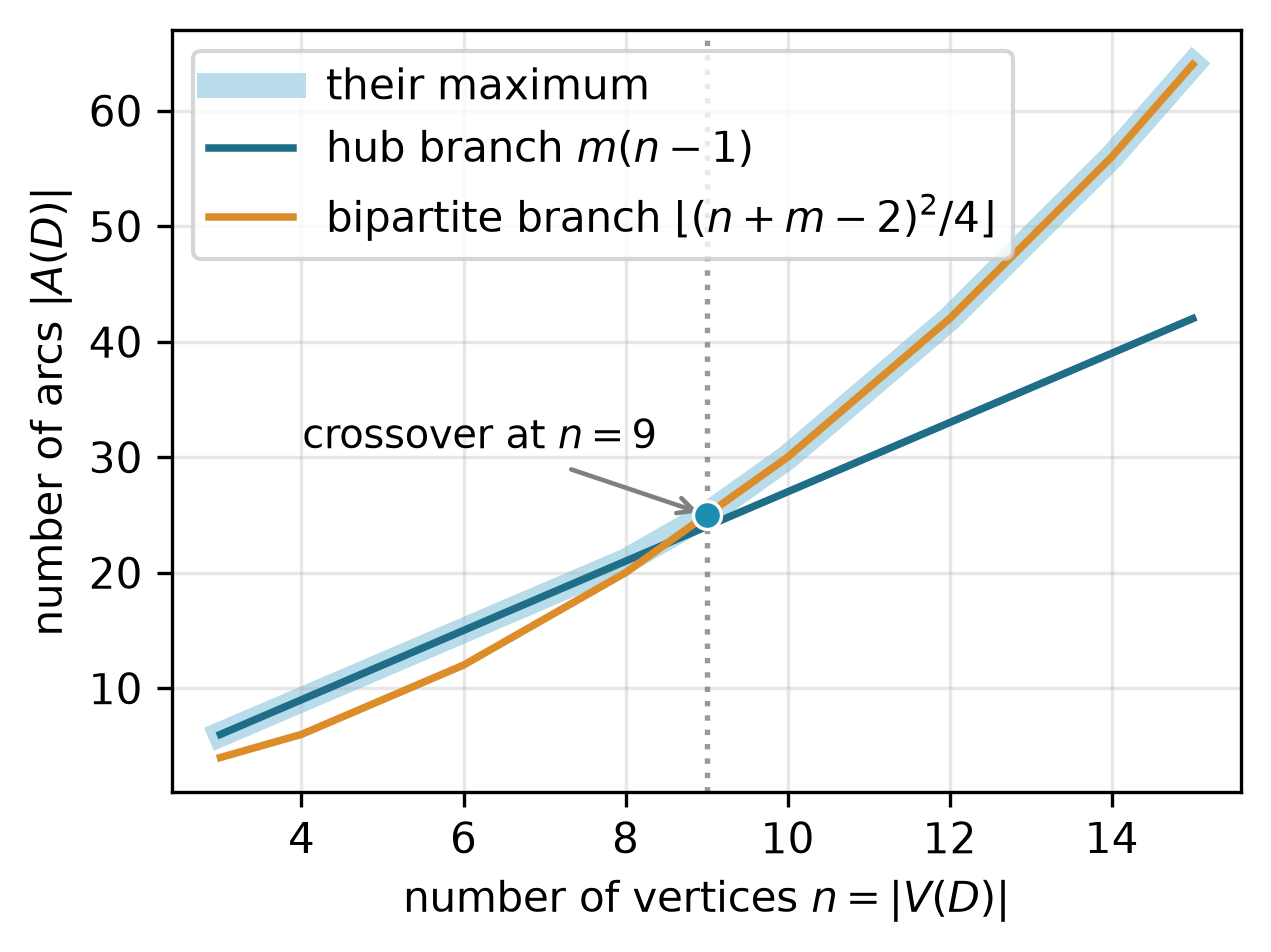
\includegraphics[width=0.78\textwidth]{figures/directed_crossover.png}
    \caption{The arc counts of the hub and of the augmented bipartite digraph at $m = 3$, and their maximum. These are lower bounds only.}
    \label{fig:crossover}
\end{figure}



\Cref{sec:status-simple-directed} discusses the asymptotics.
It is open whether the arc and vertex values are equal for $m\ge3$.
With parallel arcs allowed, \Cref{thm:dir-multi-full} gives the exact value.

\section{Why direction makes the value quadratic}

For undirected graphs the maximum is linear in $n$ (\Cref{thm:mader}).
For digraphs it is quadratic.
In \Cref{const:bipartite}, all arcs go from one part to the other, so a directed route can cross between the parts only once.
This digraph has $\floor{n^2/4}$ arcs and $\lec^{\max}=1$.
In contrast, an undirected graph with $\lec^{\max}\le1$ has no cycle, so it has at most $n-1$ edges.

\Cref{const:augmented-bipartite} extends this idea to every $m$ (\Cref{fig:augmented-wall}).
Each vertex of the larger part gets $m-2$ extra arcs from other vertices of that part.
These arcs give $m-2$ short detours.
They raise $\lec^{\max}$ to $m-1$ and the number of arcs to $\floor{(n+m-2)^2/4}$.
At $m=3$ and $n=10$, this digraph has $30$ arcs, while the hub has $27$.

\begin{figure}[t]
\centering
\begin{tikzpicture}[>=Stealth, scale=1.0,
    wallarc/.style={gdirfaint},
    cyc/.style={-{Stealth[length=2.4mm]}, line width=1.3pt, vertexorange!85!black}]

  % The m = 3, n = 10 instance: |A| = 4, |B| = 6. B is drawn as the ring its
  % m-2 = 1 cyclic in-arc per vertex actually forms, rather than as a second
  % column, where six arcs along one side merge into a single visible stroke.
  \foreach \i/\y in {1/1.65, 2/0.55, 3/-0.55, 4/-1.65} {
    \node[smallvertex] (a\i) at (0,\y) {$a_{\i}$};
  }
  \foreach \j/\ang in {1/90, 2/30, 3/-30, 4/-90, 5/-150, 6/150} {
    \node[smallvertex] (b\j) at ($(5.6,0)+(\ang:1.85)$) {$b_{\j}$};
  }
  \begin{scope}[on background layer]
    \node[draw=KULblauw1!25, fill=KULblauw1!6, rounded corners=10pt,
          fit={(a1) (a4)}, inner sep=9pt] {};
    \node[draw=vertexorange!35, fill=vertexorange!5, circle,
          fit={(b1) (b2) (b3) (b4) (b5) (b6)}, inner sep=1pt] {};
  \end{scope}
  \node[font=\scriptsize, KULblauw1] at (0,2.55) {part $A$};
  \node[font=\scriptsize, vertexorange!75!black] at (5.6,2.55) {part $B$};

  % every arc from A to B: 4 x 6 = 24
  \foreach \i in {1,...,4}{\foreach \j in {1,...,6}{\draw[wallarc] (a\i) -- (b\j);}}

  % inside B, each b_j takes its m-2 = 1 cyclic predecessor: 6 more arcs
  \foreach \j/\k in {1/2, 2/3, 3/4, 4/5, 5/6, 6/1} {
    \draw[cyc] (b\j) -- (b\k);
  }

  \node[font=\scriptsize] at (0,-2.55) {$24$ arcs $A \to B$};
  \node[font=\scriptsize, align=center, vertexorange!75!black] at (5.6,-2.55)
    {$6$ cyclic in-arcs inside $B$};
\end{tikzpicture}
\caption{The augmented bipartite digraph of \Cref{const:augmented-bipartite} at $m = 3$, $n = 10$. All arcs between the parts go from $A$ to $B$. Inside $B$, each vertex gets one arc from the previous vertex on a cycle. A pair $a_i, b_j$ has the direct arc and one detour, so $\lec^{\max} = 2$. The digraph has $24 + 6 = 30$ arcs, against $27$ for the hub.}
\label{fig:augmented-wall}
\end{figure}

An upper bound must explain why no digraph has many more arcs than this construction.
\Cref{thm:dir-arc-linear-error} shows that the optimum is at most $O_m(n)$ larger.
The linear coefficient is not known.
\Cref{prop:dir-arc-stability} also describes the shape: after deleting $O(\sqrt{m}\,n^{3/2})$ arcs, every feasible digraph has all its arcs from one part to another.

\section{Current status of the sixteen variants}

Each of the eight models has an edge problem and a vertex problem.
\Cref{tab:summary} gives an overview, and the subsections below explain it.


\begin{figure}[t]
\centering
\resizebox{\textwidth}{!}{%
\begin{tikzpicture}
  \node[vtroot, fill=KULblauw3a!18]  (root) at (9.0,3.9) {Problem 915};
  \node[vtmodel, fill=KULblauw3a!12] (simple) at (1.8,2.6)  {simple};
  \node[vtmodel, fill=KULblauw3a!12] (multi)  at (6.6,2.6)  {multi};
  \node[vtmodel, fill=KULblauw3a!12] (hyper)  at (11.4,2.6) {hyper};
  \node[vtmodel, fill=KULblauw3a!12] (mhyper) at (16.2,2.6) {multi-hyper};
  \draw[vtedge] (root) -- (simple);
  \draw[vtedge] (root) -- (multi);
  \draw[vtedge] (root) -- (hyper);
  \draw[vtedge] (root) -- (mhyper);
  \node[vtdir, fill=KULblauw3a!8]  (d0) at (0.6,1.3)  {undirected};
  \node[vtdir, fill=KULblauw3a!8]  (d1) at (3.0,1.3)  {directed};
  \node[vtdir, fill=KULblauw3a!8]  (d2) at (5.4,1.3)  {undirected};
  \node[vtdir, fill=KULblauw3a!8]  (d3) at (7.8,1.3)  {directed};
  \node[vtdir, fill=KULblauw3a!8]  (d4) at (10.2,1.3) {undirected};
  \node[vtdir, fill=KULblauw3a!8]  (d5) at (12.6,1.3) {directed};
  \node[vtdir, fill=KULblauw3a!8]  (d6) at (15.0,1.3) {undirected};
  \node[vtdir, fill=KULblauw3a!8]  (d7) at (17.4,1.3) {directed};
  \draw[vtedge] (simple) -- (d0);
  \draw[vtedge] (simple) -- (d1);
  \draw[vtedge] (multi)  -- (d2);
  \draw[vtedge] (multi)  -- (d3);
  \draw[vtedge] (hyper)  -- (d4);
  \draw[vtedge] (hyper)  -- (d5);
  \draw[vtedge] (mhyper) -- (d6);
  \draw[vtedge] (mhyper) -- (d7);
  \node[vtleaf, fill=regimeProved!16]      (l0)  at (0,0)    {edge};
  \node[vtleaf, fill=regimePartial!20]     (l1)  at (1.2,0)  {vertex};
  \node[vtleaf, fill=regimePartial!20]     (l2)  at (2.4,0)  {edge};
  \node[vtleaf, fill=regimePartial!20]     (l3)  at (3.6,0)  {vertex};
  \node[vtleaf, fill=regimeProved!16]      (l4)  at (4.8,0)  {edge};
  \node[vtleaf, fill=regimePartial!20]     (l5)  at (6.0,0)  {vertex};
  \node[vtleaf, fill=regimeProved!16]      (l6)  at (7.2,0)  {edge};
  \node[vtleaf, fill=regimePartial!20]     (l7)  at (8.4,0)  {vertex};
  \node[vtleaf, fill=regimePartial!20]     (l8)  at (9.6,0)  {edge};
  \node[vtleaf, fill=regimePartial!20]     (l9)  at (10.8,0) {vertex};
  \node[vtleaf, fill=regimeOpen!22]        (l10) at (12.0,0) {edge};
  \node[vtleaf, fill=regimeOpen!22]        (l11) at (13.2,0) {vertex};
  \node[vtleaf, fill=regimePartial!20]     (l12) at (14.4,0) {edge};
  \node[vtleaf, fill=regimePartial!20]     (l13) at (15.6,0) {vertex};
  \node[vtleaf, fill=regimeOpen!22]        (l14) at (16.8,0) {edge};
  \node[vtleaf, fill=regimeOpen!22]        (l15) at (18.0,0) {vertex};
  \draw[vtedge] (d0) -- (l0);  \draw[vtedge] (d0) -- (l1);
  \draw[vtedge] (d1) -- (l2);  \draw[vtedge] (d1) -- (l3);
  \draw[vtedge] (d2) -- (l4);  \draw[vtedge] (d2) -- (l5);
  \draw[vtedge] (d3) -- (l6);  \draw[vtedge] (d3) -- (l7);
  \draw[vtedge] (d4) -- (l8);  \draw[vtedge] (d4) -- (l9);
  \draw[vtedge] (d5) -- (l10); \draw[vtedge] (d5) -- (l11);
  \draw[vtedge] (d6) -- (l12); \draw[vtedge] (d6) -- (l13);
  \draw[vtedge] (d7) -- (l14); \draw[vtedge] (d7) -- (l15);
  % Legend, one row in the order of the caption: known, partial, open.
  \node[vtleaf, fill=regimeProved!16, minimum width=8mm]  (leg1) at (0,-1.5) {};
  \node[anchor=west, font=\scriptsize] at (0.6,-1.5) {exact value known for every $m$};
  \node[vtleaf, fill=regimePartial!20, minimum width=8mm] (leg2) at (5.2,-1.5) {};
  \node[anchor=west, font=\scriptsize] at (5.8,-1.5) {exact value known for some $m$ or on a stated range};
  \node[vtleaf, fill=regimeOpen!22, minimum width=8mm]    (leg3) at (14.0,-1.5) {};
  \node[anchor=west, font=\scriptsize] at (14.6,-1.5) {only the leading term is known};
\end{tikzpicture}%
}
\caption{Overview of the sixteen variants. Blue: the exact value is known for every $m$. Purple: the exact value is known for some $m$ or on a stated range. Amber: only the leading term is known.}
\label{fig:variant-tree-status}
\end{figure}

\begin{table}[htbp]
\centering\small
\renewcommand{\arraystretch}{1.2}
\begin{tabularx}{\textwidth}{@{}>{\raggedright\arraybackslash}p{0.19\textwidth}>{\raggedright\arraybackslash}X>{\raggedright\arraybackslash}X@{}}
\toprule
Model & Edge or arc separation & Vertex separation \\
\midrule
Simple graph & $\floor{m(n-1)/2}$ for $n\ge m$ & Exact for $m\le5$. Open for $m\ge6$ \\
Multigraph & $(m-1)(n-1)$ & $n-1$ at $m=2$, $2(n-1)$ at $m=3$. Open for $m\ge4$ \\
Simple hypergraph & At most $\floor{(m-1)(n-1)/(r-1)}$, equal when $m-1\le\binom{n-2}{r-2}$ & $\floor{(n-1)/(r-1)}$ at $m=2$, $\floor{2(n-1)/(r-1)}$ at $m=3$ for $r<n$. Open for $m\ge4$ \\
Multihypergraph & At most $\floor{(m-1)(n-1)/(r-1)}$, equal when $(r-1)\mid(n-1)$ & $\floor{(n-1)/(r-1)}$ at $m=2$. At $m=3$ at most $\floor{2(n-1)/(r-1)}$, equal when $(r-1)\mid(n-1)$ \\
Simple digraph & $M(n)$ at $m=2$. $n^2/4+\Theta_m(n)$ for $m\ge3$ & Same \\
Directed multigraph & $(m-1)M(n)$ & $M(n)$ at $m=2$. $(m-1)n^2/4+O_m(n)$ \\
Directed simple hypergraph & $(1+o(1))(m-1)n^2/(4(r-1))$ & Same \\
Directed multihypergraph & $(1+o(1))(m-1)n^2/(4(r-1))$ & Same \\
\bottomrule
\end{tabularx}
\caption{Status of the sixteen problems. Here $m\ge2$, hypergraphs have $r\ge3$, and asymptotic statements are for fixed $m$ and $r$ as $n\to\infty$.}
\label{tab:summary}
\end{table}

\subsection{Simple undirected graphs}
\label{sec:status-simple-undirected}

For edge separation, the answer is known for all $n$:
\[
 \ell_m(n)=
 \begin{cases}
 \binom n2,&n<m,\\
 \floor{m(n-1)/2},&n\ge m.
 \end{cases}
\]
For $n<m$ the complete graph is feasible. For $n\ge m$, the hub-and-spokes graph attains Mader's bound.
The Gomory--Hu proof shows why simplicity matters: at most $n-1$ edges cross only one tree edge, and every other edge crosses at least two (\Cref{thm:mader,thm:extremal-existence}).

For vertex separation, the edge formula is still exact for $m\le4$.
At $m=5$ the two values agree up to $n=13$, but from $n=14$ the vertex value is $\floor{8n/3}-4$.
The first difference is $33$ against $32$ at $n=14$ (\Cref{thm:leonard,thm:sorensen-thomassen}).

For $m\ge6$ the vertex value is open.
\Cref{thm:simple-vertex-blocks} reduces it to a choice of $2$-connected blocks, with a limiting rate $c_m$.
Known results give $c_m=m/2$ for $m\le4$ and $c_5=8/3$ (\Cref{thm:sorensen-thomassen}).
For $m\ge6$ they give $m/2<c_m\le2(m-1)$.

\subsection{Undirected multigraphs}
\label{sec:status-multigraph}

For edge separation the value is $L_m(n)=(m-1)(n-1)$, attained by a tree with every edge repeated $m-1$ times (\Cref{thm:multigraph-edge}).

For vertex separation, parallel edges count as separate routes, so the problem differs from the simple one.
\Cref{lem:multi-vertex-split} splits $\kap(u,v)$ into the parallel edges and the longer routes.
At $m=2$ this forces a forest without repeated edges, so $K_2(n)=n-1$.
At $m=3$, the incidence-rank bound and a doubled tree give $K_3(n)=2(n-1)$ (\Cref{thm:hyper-vertex-m3,prop:hyper-vertex-lower-multi}).
At $m=5$ the thickened theta gives $K_5(4)\ge14>12=L_5(4)$ (\Cref{sec:multi-vertex}).

The block reduction shows how a good small block can be repeated.
Thickened complete graphs and thickened complete bipartite graphs give bounds of order $m^2n$ as $m\to\infty$ and $n/m\to\infty$.
The constants are $3-2\sqrt2$ below and $2$ above. The true constant is not known.

\subsection{Simple undirected hypergraphs}
\label{sec:status-simple-hypergraph}

In an $r$-uniform hypergraph one hyperedge joins several vertices, but it can carry only one route of an edge-disjoint family.
The edge bound is
\[
 \ell_m^{(r)}(n)\le\floorfrac{(m-1)(n-1)}{r-1}.
\]
It is attained when $m-1\le\binom{n-2}{r-2}$, that is, when there are enough different hyperedges (\Cref{prop:hyper-edge,thm:simple-hyper-edge}).
This condition matters: at $n=r=m=3$ there is only one possible hyperedge, while the bound is two.

For vertex separation, $k_2^{(r)}(n)=\floor{(n-1)/(r-1)}$.
Here feasibility means that the incidence graph is a forest, and a star hypertree attains the bound.
At $m=3$ the incidence-rank bound gives $\floor{2(n-1)/(r-1)}$, attained by simple hypergraphs for $2<r<n$.
For $m\ge4$ the vertex problem is open.
The edge bound does not help here, because the vertex condition is weaker.

\subsection{Undirected multihypergraphs}
\label{sec:status-multihypergraph}

The edge bound also holds when hyperedges repeat.
A star hypertree with every hyperedge repeated $m-1$ times attains $(m-1)(n-1)/(r-1)$ when $r-1$ divides $n-1$.
At $n=r=m=3$, two copies of the only hyperedge reach the bound, which no simple hypergraph can do.
Repeated hyperedges can also reach the bound in other cases: the construction with twelve hyperedges at $(n,m,r)=(6,6,3)$ meets the bound $12$ (\Cref{const:multihyper-six}).

For vertex separation, repeated hyperedges do not help at $m=2$, because two copies of a hyperedge already give two separated routes.
So the value is again $\floor{(n-1)/(r-1)}$.
At $m=3$ the upper bound is the same as for simple hypergraphs.
A star hypertree with every hyperedge doubled attains it when $r-1$ divides $n-1$ (\Cref{prop:hyper-vertex-lower-multi}).
For $m\ge4$ the vertex problem is open.


\subsection{Simple directed graphs}
\label{sec:status-simple-directed}

In a digraph, the one-way bipartite digraph already has $\floor{n^2/4}$ arcs with $\lec^{\max}=1$.
At $m=2$ the value under both separations is $M(n)=\max(2(n-1),\floor{n^2/4})$.
The proof uses the reachability skeleton.

For fixed $m\ge3$, both values are $n^2/4+\Theta_m(n)$.
The upper bound also follows from a theorem of Huang and Lyu \cite[Theorem~2]{HuangLyu26} with $t=m-1$.
A feasible digraph has at most $m-1$ paths of length two between any two vertices, since paths with different midpoints are internally vertex-disjoint.
Their theorem then gives $|A|\le n^2/4+(m-1)n+O_m(1)$ for large $n$.
The augmented bipartite digraph gives $n^2/4+(m-2)n/2+O_m(1)$ from below.
\Cref{thm:dir-arc-linear-error} gives an elementary proof, with a bound that holds for every $n$.

The exact value and the linear coefficient are open.
It is also open whether the arc and vertex values are equal for $m\ge3$.
An upper bound for the arc problem does not bound the vertex problem, because more digraphs are vertex-feasible.

\subsection{Directed multigraphs}
\label{sec:status-directed-multigraph}

For arc separation the value is $L_m^{\mathrm{dir}}(n)=(m-1)M(n)$.
The proof removes a reachability skeleton $m-1$ times.
A bidirected tree and the one-way bipartite digraph, with every arc repeated $m-1$ times, attain the two terms.
For $n\ge\max(8,2m)$ the bipartite construction is the only extremal multigraph (\Cref{thm:dir-multi-uniqueness}).

For vertex separation the answer can be larger.
On three vertices, take every arc with multiplicity $4$.
Every route of length at least two passes through the third vertex, so $\kap\le4+1=5$.
This digraph has $24$ arcs, so $K_6^{\mathrm{dir}}(3)\ge24$, while $L_6^{\mathrm{dir}}(3)=20$.
For fixed $m$, the shadow bound at $r=2$ and the bipartite construction give $K_m^{\mathrm{dir}}(n)=(m-1)n^2/4+O_m(n)$ (\Cref{thm:dir-hyper-constant,cor:dir-multi-incidence}).
The exact value is open. A block construction gives a lower bound (\Cref{prop:dir-multi-vertex-blocks}).



\subsection{Simple directed hypergraphs}
\label{sec:status-directed-simple-hypergraph}

In the forward model a hyperedge has one tail and $r-1$ heads.
For fixed $r\ge3$ and $m\ge2$, the leading term under both separations is $(m-1)n^2/(4(r-1))$.
The upper bound uses the shadow digraph.
The lower bound uses a two-layer construction: all tails on one side, all heads on the other (\Cref{prop:dir-hyper-first}).

For small $n$ there may not be enough different head sets for this construction.
Then another construction can be larger: give every vertex the same number of outgoing hyperedges.
For example, at $n=m=6$ and $r=3$, every vertex gets five outgoing hyperedges, which gives $30$ hyperedges.
All routes from a vertex start with one of its five outgoing hyperedges, so the hypergraph is feasible (\Cref{const:bounded-outdegree-hyper}).


\subsection{Directed multihypergraphs and orientation choices}
\label{sec:status-directed-multihypergraph}\label{sec:orientation-models}

With repeated hyperedges, the two-layer construction no longer needs different head sets.
The leading term is still $(m-1)n^2/(4(r-1))$ under both separations.
At $r=2$ these are the directed multigraphs.
For simple digraphs ($r=2$) the leading coefficient is $1/4$ instead, so the simple case needs $r\ge3$.

We can also orient a hyperedge in other ways.
In the \emph{backward} model a hyperedge has one head and $r-1$ tails.
Reversing all arcs turns it into the forward model (\Cref{lem:dir-hyper-duality}).
In the \emph{general} model a hyperedge is split in any way into a non-empty set of tails and a non-empty set of heads.
All three models have the same leading term (\Cref{thm:dir-hyper-general-constant}).
It is open whether the forward and general models have the same exact values.





\section{Scope of the program}

The program measures connectivity in all sixteen variants with one max-flow checker.
It uses tabu search and simulated annealing for graphs, and random greedy growth for hypergraphs.
An exhaustive search gives an exact value only when it covers every candidate or excludes it by a correct pruning rule.
A heuristic search only gives lower bounds.



\section{Open problems}

Four directions remain open.
\begin{itemize}
\item For directed graphs, determine the exact values, linear corrections and
extremal structures, including whether the two separations agree in the simple model.
\item For undirected vertex separation, determine the simple value at $m\ge6$
and the multigraph value at $m\ge4$, including the best blocks and growth rates.
\item For undirected hypergraphs, determine edge attainment outside the range
where it is established and find vertex bounds beyond the $m=3$ rank argument.
\item For directed hypergraphs, determine finite values and compare the effects
of multiplicity, separation and orientation beyond the established leading term.
\end{itemize}
Three concrete open questions:
\begin{enumerate}
\item Find $\ell_m^{\mathrm{dir}}(n)$ for $m\ge3$.
\item Is $k_m^{\mathrm{dir}}(n)=\ell_m^{\mathrm{dir}}(n)$ for $m\ge3$?
\item Is $K_4(n)=L_4(n)=3(n-1)$ for every $n$?
\end{enumerate}
